%% Introducción



\documentclass[serif, aspectratio=169]{beamer}
\usepackage{bookmark}
%\documentclass[serif]{beamer}  % for 4:3 ratio
\usepackage[T1]{fontenc} 
\usepackage{fourier}
\usepackage{hyperref}
\usepackage{bookmark}
\usepackage{latexsym,amsmath,xcolor,multicol,booktabs,calligra}
\usepackage{graphicx,listings,stackengine}
\usepackage[spanish]{babel}
%\setbeameroption{show notes on second screen=right} % Para la versión final desactivo esto.

\author{Alberto Daniel Lange}
\vspace{-3mm}
\title{Sistema de comunicaciones seguras \\ con segmentación virtual de dominios}
\subtitle{\small Avance de proyecto}
\institute{
    Dirección: Juan Ignacio Vaccarezza \\
    Codirección: Santiago Pérez Ghiglia \\
    \vspace{2mm}
    Ingeniería en Telecomunicaciones \\
    Instituto Balseiro
}
\vspace{-7mm}
\date{\small 26 de febrero de 2025}
\usepackage{UoWstyle}

% defs
\def\cmd#1{\texttt{\color{red}\footnotesize $\backslash$#1}}
\def\env#1{\texttt{\color{blue}\footnotesize #1}}
\definecolor{deepblue}{rgb}{0,0,0.5}
\definecolor{deepred}{RGB}{153,0,0}
\definecolor{deepgreen}{rgb}{0,0.5,0}
\definecolor{halfgray}{gray}{0.55}

\lstset{
    basicstyle=\ttfamily\small,
    keywordstyle=\bfseries\color{deepblue},
    emphstyle=\ttfamily\color{deepred},   
    stringstyle=\color{deepgreen},
    numbers=left,
    numberstyle=\small\color{halfgray},
    rulesepcolor=\color{red!20!green!20!blue!20},
    frame=shadowbox,
}


\begin{document}

% INICIO
\begin{frame} % LOGOS INSTITUCIONALES
    \titlepage
    \vspace*{-0.8cm}
\begin{columns}
    \begin{column}{0.25\textwidth}
        \begin{figure}
            \centering
            
\includegraphics[width=0.3\textwidth]{images/institucionales_cnea.png}
        \end{figure}
    \end{column}
    \begin{column}{0.25\textwidth}
        \begin{figure}
            \centering
            
\includegraphics[width=0.3\textwidth]{images/institucionales_IB.png}
        \end{figure}
    \end{column}
    \begin{column}{0.25\textwidth}
        \begin{figure}
            \centering
            
\includegraphics[width=0.5\textwidth]{images/institucionales_INVAP.png}
        \end{figure}
    \end{column}
    \begin{column}{0.25\textwidth}
        \begin{figure}
            \centering
            
\includegraphics[width=0.3\textwidth]{images/institucionales_cuyo.png}
        \end{figure}
        
    \end{column}
\end{columns}
\end{frame}


\begin{frame}    
\tableofcontents[sectionstyle=show,
subsectionstyle=show/shaded/hide,
subsubsectionstyle=show/shaded/hide]
\end{frame}

\section{Introducción}

\begin{frame}{Contexto}
            \begin{figure}
                \centering
                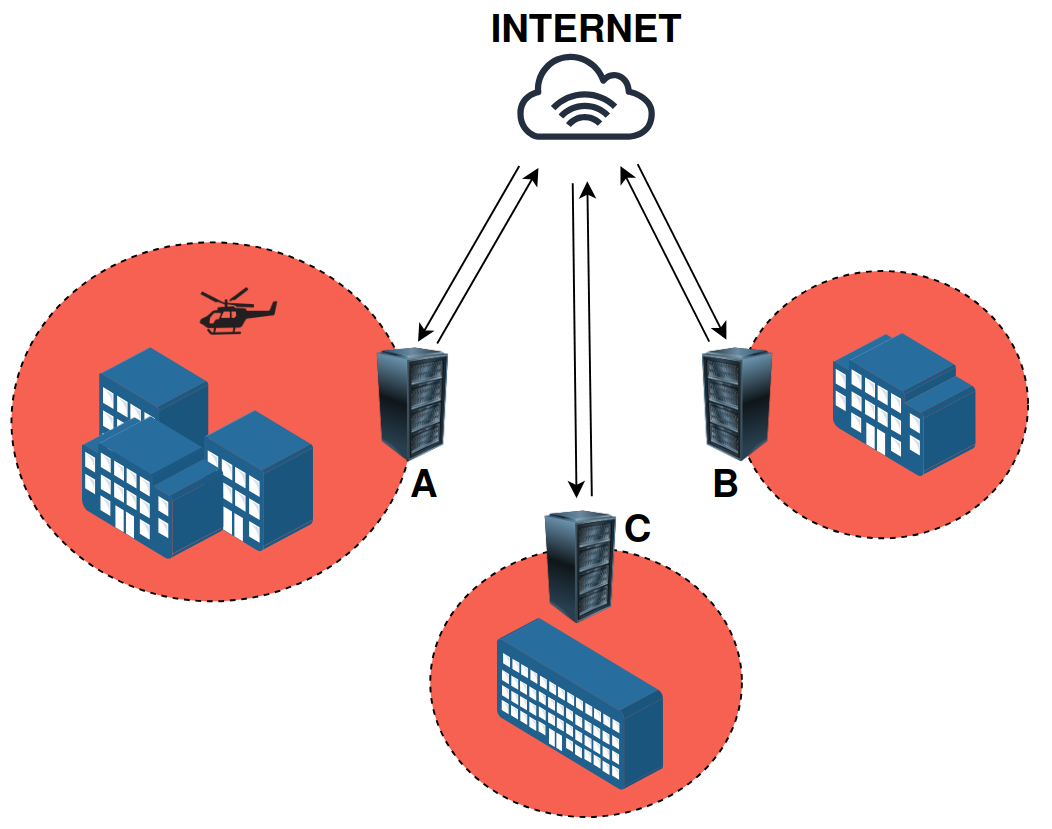
\includegraphics[width=0.5\textwidth]{images/conops.png}
                \caption{\centering Esquema simplificado de operación del sistema.}
            \end{figure}

    \note{Antes que nada quiero dar un pantallazo general de lo que se trata este proyecto. ¿A que nos referimos con sistema de comunicaciones seguras? Se trata del desarrollo de un dispositivo encriptador destinado a asegurar las comunicaciones entre sitios, es decir, que permita establecer una red privada virtual o VPN entre estos sitios.
    En la figura se puede ver un esquema simplificado de la operación del sistema. Estos dispositivos hacen de interfaz entre dos dominios, el rojo, que contiene información no cifrada, y el negro, que es la parte externa, donde la información se encuentra cifrada.
    }
\end{frame}


\begin{frame}{Progreso alcanzado anteriormente}
    \begin{columns}
    \begin{column}{0.33\textwidth}

    \begin{itemize}
        \item Definición y validación de arquitectura lógica en laboratorio virtual.
    \end{itemize}

    \end{column}
    \begin{column}{0.7\textwidth}
    \begin{figure}
        \centering
        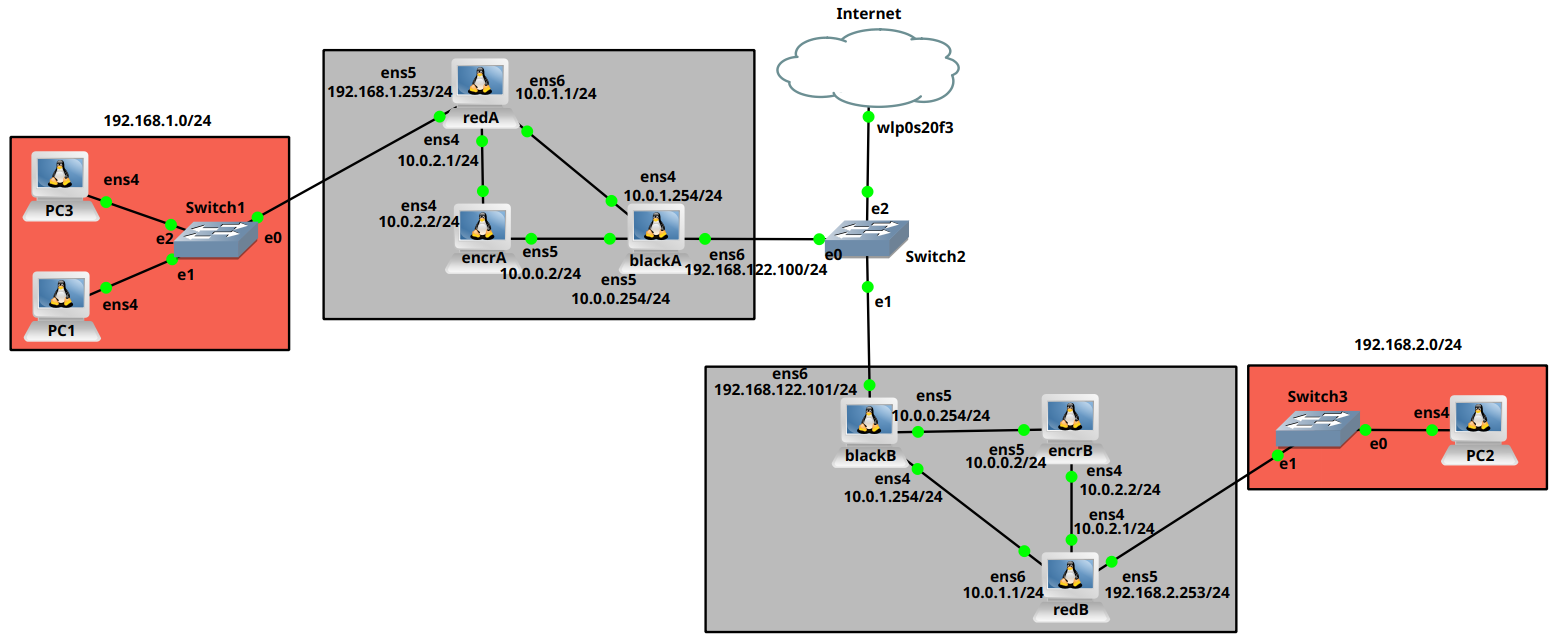
\includegraphics[width=0.95\textwidth]{images/gns3_2.png}
        \caption{Implementación de la propuesta de solución en GNS3.} 
    \end{figure}
    \end{column}
\end{columns}
\end{frame}

\begin{frame}{Pendientes}
    \begin{itemize}
        \item Validación del encriptador en ambiente virtualizado. 
        \item Implementación sobre hardware.
    \end{itemize}

\end{frame}

\section{Revisión bibliográfica}

\begin{frame}{seL4}
    \begin{columns}
        \begin{column}{0.35\textwidth}
            \begin{itemize}
                \item Microkernel de código abierto.
                \item Formalmente probado.
                \item Hipervisor tipo 1.
                \item Aislamiento garantizado entre componentes.
            \end{itemize}
        \end{column}

        \begin{column}{0.6\textwidth}
            \begin{figure}
                \centering
                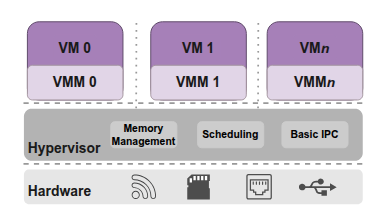
\includegraphics[width=\textwidth]{images/sel4scheme.png}
                \caption{\centering Arquitectura de seL4. (algo así, otra imagen)} 
            \end{figure}
        \end{column}
    \end{columns}
    
    \note{seL4 es un microkernel diseñado para ser seguro, eficiente y confiable. Se ejecuta directamente sobre hardware con capacidad de funcionar como hipervisor de tipo 1. Su característica más importante es la verificación formal de su funcionamiento, lo que significa que se demostró matemáticamente que su implementación cumple con sus especificaciones de diseño. Una de estas especificaciones críticas es la aislación entre componentes, fundamental para nuestro sistema de segmentación de dominios.}
\end{frame}

\begin{frame}{CAmkES}
    \begin{columns}
        \begin{column}{0.5\textwidth}
            \begin{itemize}
                \item \textbf{C}omponent \textbf{A}rchitecture for \textbf{m}icro\textbf{k}ernel-based \textbf{E}mbedded \textbf{S}ystems.
                \item Framework de desarrollo para seL4.
                \item Arquitectura basada en componentes.
                \item Comunicación mediante interfaces bien definidas.
            \end{itemize}
        \end{column}

        \begin{column}{0.5\textwidth}
            \begin{figure}
                \centering
                \includegraphics[width=0.8\textwidth]{example-image}
                \caption{\centering Arquitectura de componentes CAmkES.} 
            \end{figure}
        \end{column}
    \end{columns}
    
    \note{CAmkES es un framework que simplifica el desarrollo de sistemas sobre seL4. Permite diseñar aplicaciones como un conjunto de componentes que se comunican a través de interfaces bien definidas. Esto es especialmente útil para nuestro proyecto ya que cada máquina virtual puede ser vista como un componente independiente con interfaces de comunicación controladas, lo que facilita la implementación de la segmentación de dominios.}
\end{frame}

\begin{frame}{Modelo minimal\_64}
    \begin{columns}
        \begin{column}{0.5\textwidth}
            \begin{itemize}
                \item Ejemplo básico de CAmkES.
                \item Implementación mínima de una VM para arquitectura de 64 bits.
                \item Punto de partida para el desarrollo.
            \end{itemize}
        \end{column}

        \begin{column}{0.5\textwidth}
            \begin{figure}
                \centering
                \includegraphics[width=0.9\textwidth]{example-image}
                \caption{\centering Arquitectura minimal\_64.} 
            \end{figure}
        \end{column}
    \end{columns}
    
    \note{El modelo minimal_64 es un ejemplo fundamental en CAmkES que proporciona una configuración básica para ejecutar máquinas virtuales de 64 bits sobre seL4. Este modelo incluye los componentes esenciales como el VMM (Virtual Machine Monitor) y una configuración mínima de red. Nos sirve como base para entender cómo estructurar nuestro sistema y como punto de partida antes de agregar la complejidad de la comunicación ZeroMQ y la funcionalidad de encriptación.}
\end{frame}

\begin{frame}{Modelo zmq\_samples}
    \begin{columns}
        \begin{column}{0.5\textwidth}
            \begin{itemize}
                \item Comunicación entre máquinas virtuales usando ZeroMQ.
                \item Base para la implementación del encriptador.
            \end{itemize}
        \end{column}

        \begin{column}{0.5\textwidth}
            \begin{figure}
                \centering
                \includegraphics[width=0.9\textwidth]{example-image}
                \caption{\centering Arquitectura zmq\_samples.} 
            \end{figure}
        \end{column}
    \end{columns}
    
    \note{El modelo zmq_samples es un ejemplo práctico que demuestra cómo implementar comunicación segura entre máquinas virtuales en seL4 usando ZeroMQ. Este modelo nos sirve como punto de partida para implementar la comunicación entre los dominios rojo y negro de nuestro encriptador, manteniendo el aislamiento necesario mientras permite el intercambio controlado de información.}
\end{frame}



\section{Desarrollo}

\begin{frame}{Estrategia de modelos en entornos virtualizados}
   \begin{itemize}
       \item \textbf{¿Qué?}: Realizar modelos que validen progresivamente los componentes desarrollados.
       \item \textbf{¿Para qué?}: 
       \begin{itemize}
        \item Ligar problemas concretos a cada modelo y resolverlos de forma independiente.
        \item Implementar un encriptador funcional en un entorno virtualizado como paso previo a su despliegue en hardware.
       \end{itemize}
       
   \end{itemize}
\end{frame}

\begin{frame}{Modelo I: Introduciendo la arquitectura lógica}
    \begin{columns}
        \begin{column}{0.35\textwidth}
            \begin{itemize}
                \item Validar la arquitectura lógica de tres VMs.
                \item Funcionalidad \textit{split-tunneling}.
            \end{itemize}
        \end{column}
        \begin{column}{0.6\textwidth}
            \begin{figure}
                \centering
                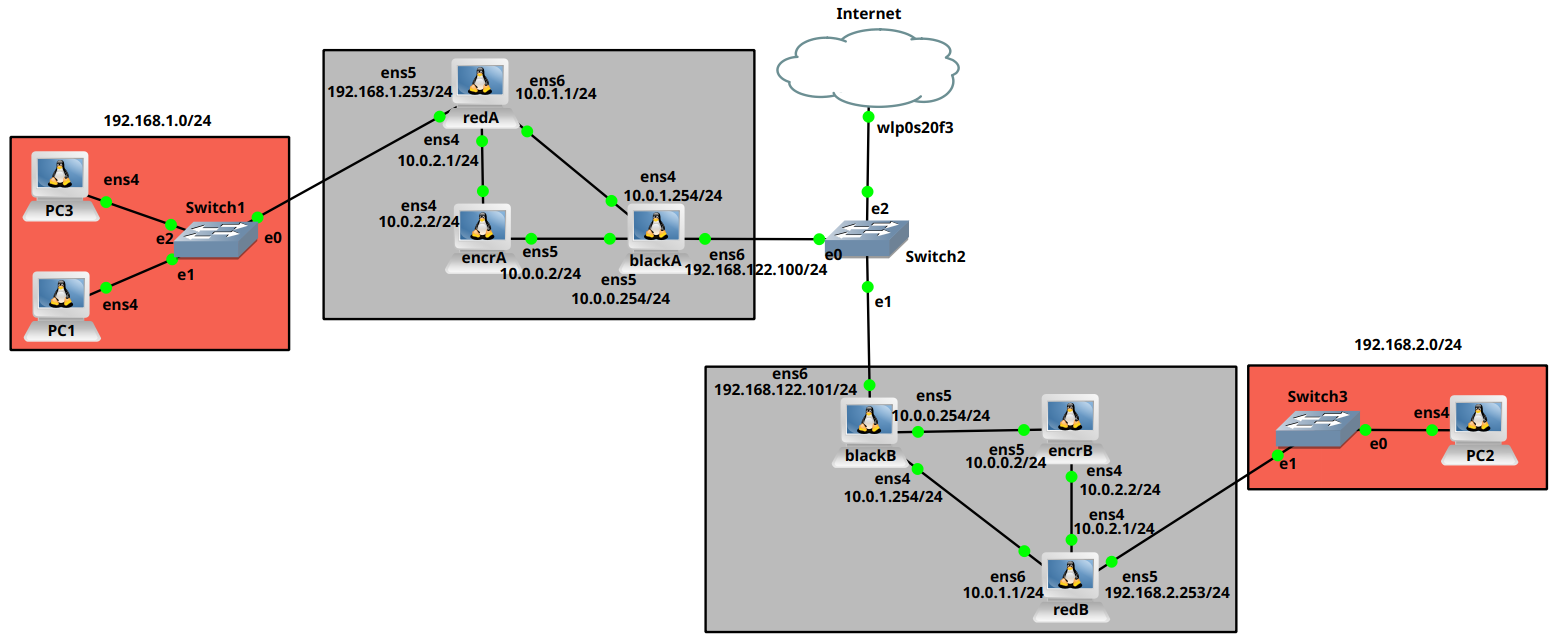
\includegraphics[width=\textwidth]{images/gns3_2.png}
                \caption{Arquitectura lógica en GNS3.}
            \end{figure}
        \end{column}
    \end{columns}
\end{frame}

\begin{frame}{Modelo II: comunicando sitios con WireGuard}
    \begin{columns}
        \begin{column}{0.35\textwidth}
            \begin{itemize}
                \item Validación del kernel Linux 4.9 con soporte para WireGuard.
                \item Obtener parámetros PCI necesarios para el passthrough de la interfaz de red.
            \end{itemize}
        \end{column}
        \begin{column}{0.6\textwidth}
            \begin{figure}
                \centering
                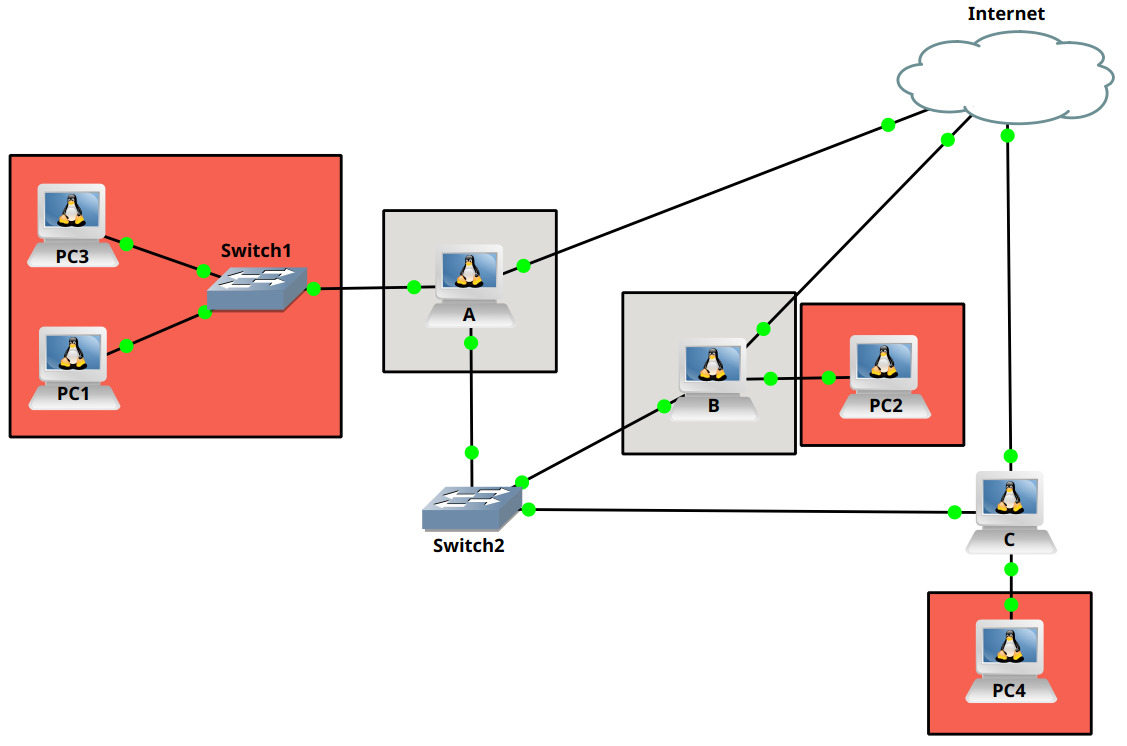
\includegraphics[width=\textwidth]{images/gns3_1.png}
                \caption{Arquitectura lógica en GNS3.}
            \end{figure}
        \end{column}
    \end{columns}
\end{frame}

\begin{frame}{Modelo II: comunicando sitios con WireGuard - Sistema operativo VMs}
        \begin{itemize}
            \item Buildroot como sistema de archivos.
            \item Kernel Linux 4.9.337.
            \item Parche de compatibilidad WireGuard con Linux $\leq$ 5.6.
        \end{itemize}
\end{frame}

\begin{frame}{Modelo III: utilizando seL4 como hipervisor}
    \begin{columns}
        \begin{column}{0.4\textwidth}
            \begin{itemize}
                \item Validación del passthrough de hardware y la compatibilidad del kernel Linux 4.9 con seL4.
            \end{itemize}
        \end{column}
        \begin{column}{0.6\textwidth}
            \begin{figure}
                \centering
                \includegraphics[width=0.5\textwidth]{example-image}
                \caption{Algo}
            \end{figure}
        \end{column}
    \end{columns}
\end{frame}

\begin{frame}{Modelo III: utilizando seL4 como hipervisor - Passthrough de hardware}
    CAmkES actúa de interfaz para la configuración del passthrough de dispositivos PCI a una VM a través de los Base Address Registers (BARs) e interrupciones.
    
    \vspace*{1cm}

     \begin{block}{\small Ejemplo de configuración en CAmkES:}
          \texttt{vm0.vm\_ioports = [start, end];} \\
          \texttt{vm0.pci\_devices = [bus, device, function, memory];} \\
          \texttt{vm0.vm\_irqs = [source, dest];}
     \end{block}
\end{frame}

\begin{frame}{Modelo III: utilizando seL4 como hipervisor - Gestión de memoria VMs}
    \texttt{simple\_untypedN\_pool:} prealocación de memoria para las VMs. \\
    \texttt{heap\_size:} tamaño del heap del VMM. \\
    \texttt{guest\_ram\_mb:} tamaño de la RAM asignada a cada VM.
\end{frame}

\begin{frame}{Modelo IV: implementando el encriptador en seL4}
    \begin{columns}
        \begin{column}{0.4\textwidth}
            \begin{itemize}
                \item Solución completa como paso previo a la implementación en hardware.
        
            \end{itemize}
        \end{column}
        \begin{column}{0.6\textwidth}
            \begin{figure}
                \centering
                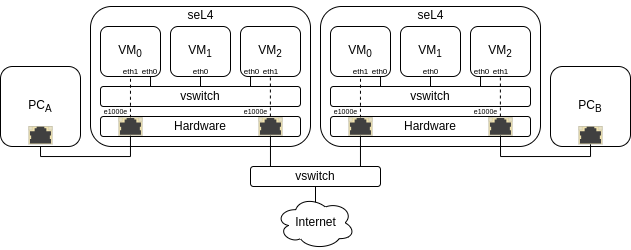
\includegraphics[width=\textwidth]{images/3_model4.png}
                \caption{Algo.}
            \end{figure}
        \end{column}
    \end{columns}
\end{frame}

\begin{frame}{Modelo IV: Encriptador en seL4 - Comunicación entre VMs}
\textbf{¿Cómo funciona?}
\begin{block}{\small Virtio-Net en VM}

\begin{itemize}
    \item El host implementa un dispositivo PCI virtual (virtio-net).
    \item La VM encuentra este dispositivo y carga el driver virtio-net.
    \item En la transmisión, la VM escribe los datos a enviar en un buffer asociado a una cola del hipervisor. El VMM notifica al host que hay datos listos en la cola (virtqueue).
\end{itemize}
\end{block}

\begin{block}{\small Virtio-Net en host}
\begin{itemize}
    \item El host lee el paquete de la virtqueue y lo copia a un buffer dentro del espacio de memoria de la VM destino.
    \item El host inyecta una interrupción en la VM destino para notificarle que hay datos disponibles.
\end{itemize}
\end{block}



\end{frame}

\begin{frame}{Modelo IV: Encriptador en seL4 - Integración}
% Mostrar ping entre PCs
\begin{figure}
    \centering
    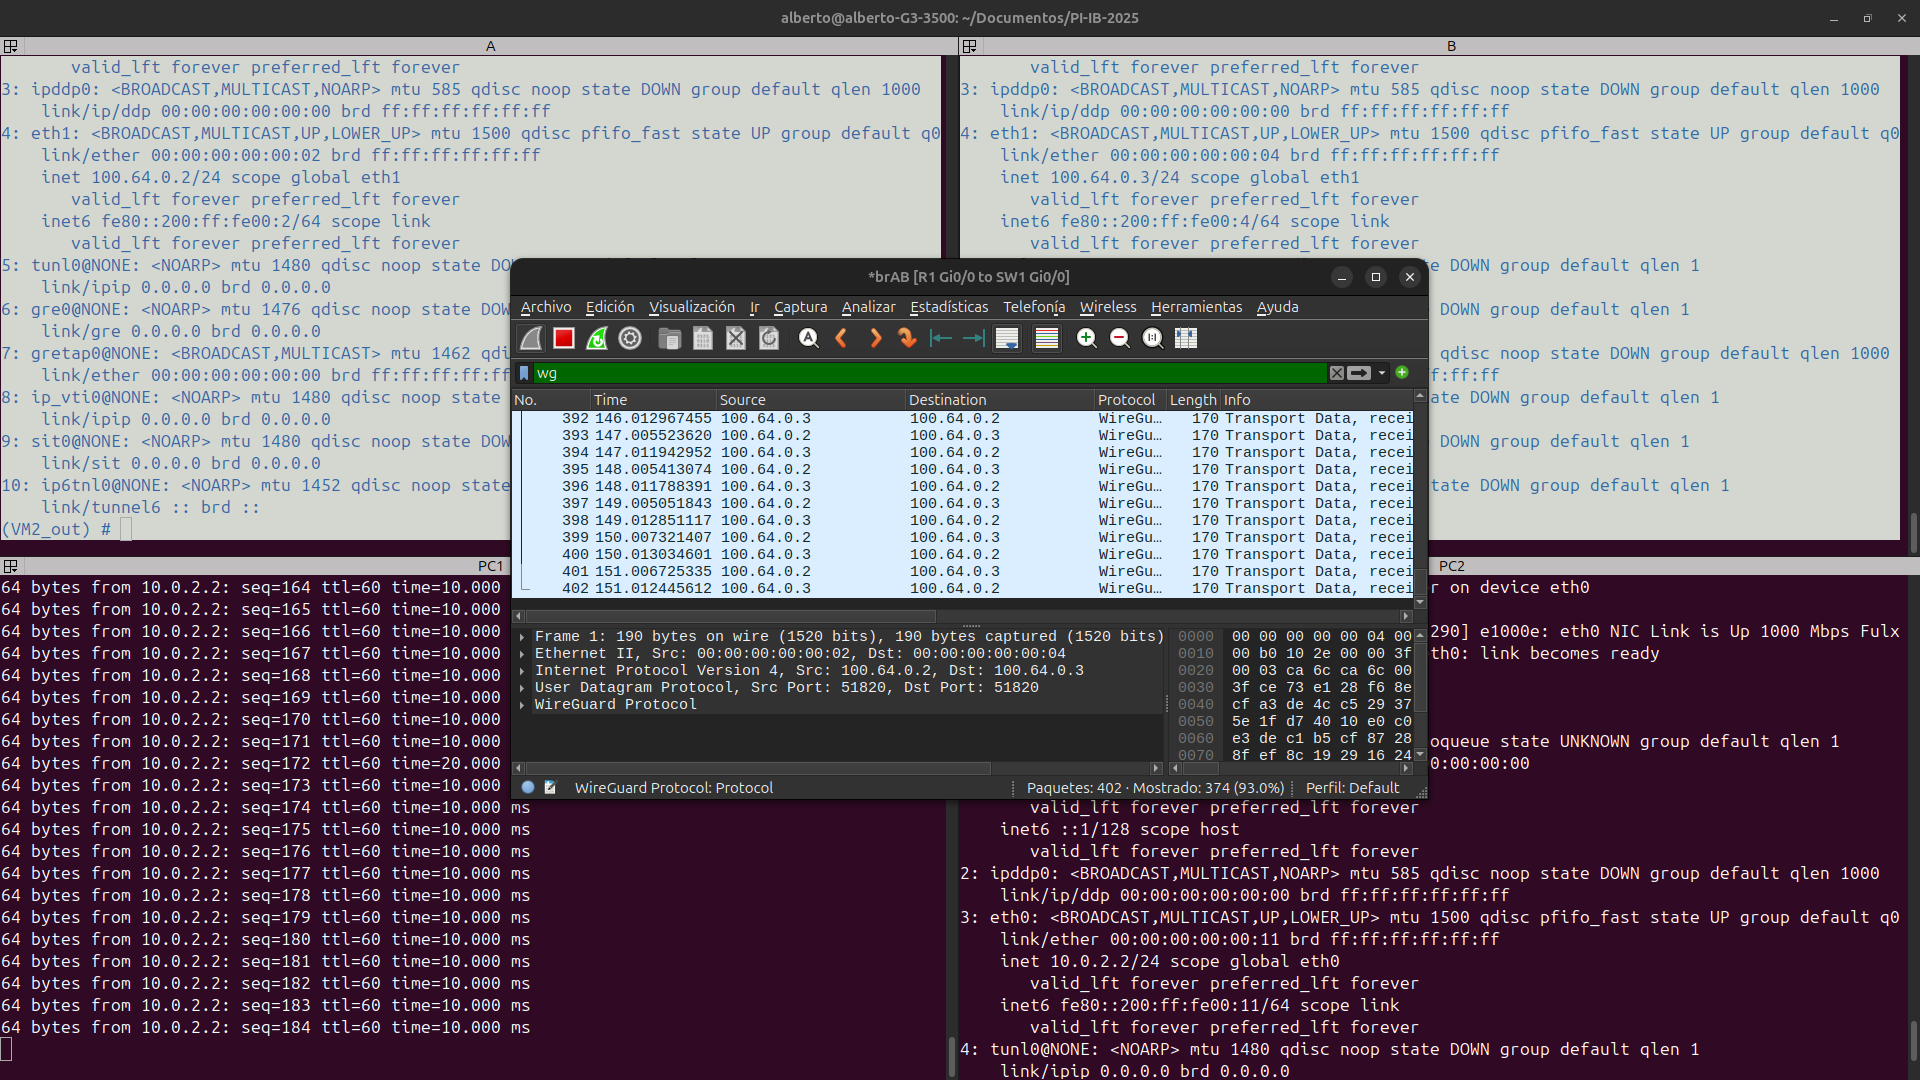
\includegraphics[width=0.8\textwidth]{images/pingAB.png}
    \caption{Ping entre PCs.}
\end{figure}
\end{frame}

\begin{frame}{Implementación en hardware}
\begin{columns}
\onslide<1->{
    \begin{column}{0.5\textwidth}
            \begin{figure}
                \centering
                \includegraphics[width=0.8\textwidth]{example-image}
                \caption{SuperMicro SYS-E300-9D.} 
            \end{figure}
        \end{column}
}
 \onslide<2->{
        \begin{column}{0.4\textwidth}
            \textbf{Desafíos:}
            \begin{itemize}
                \item[\space \textcolor{green}{\checkmark}] Redirección de consola.
                \item[{\color{red}\texttimes}] Passthrough de controlador Ethernet.
                \item[{\color{red}\texttimes}] Throughput entre VMs.
            \end{itemize}
        \end{column}
 }
\end{columns}

\end{frame}


\section{Conclusiones}
\begin{frame}{Conclusiones}
    \begin{itemize}
        \item Algo
    \end{itemize}

    \note{En resumen, hemos avanzado significativamente en el desarrollo de un sistema de comunicaciones seguras con segmentación virtual de dominios. Hemos validado la arquitectura lógica y la funcionalidad de los modelos, lo que nos permite avanzar hacia la implementación en hardware y las pruebas de integración.}
\end{frame}

\begin{frame}
    \begin{center}
        \Huge ¡Muchas gracias! \\
        \Huge ¿Preguntas?
    \end{center}
\end{frame}

% FIN

\end{document}